% Options for packages loaded elsewhere
\PassOptionsToPackage{unicode}{hyperref}
\PassOptionsToPackage{hyphens}{url}
%
\documentclass[
  11pt,
a4paper
]{article}

\usepackage{amsmath,amssymb}

% `\floatfoot' environment for notes in floats.
\usepackage{floatrow}

\usepackage{lmodern}
\usepackage{ifxetex,ifluatex}
\ifnum 0\ifxetex 1\fi\ifluatex 1\fi=0 % if pdftex
  \usepackage[T1]{fontenc}
  \usepackage[utf8]{inputenc}
  \usepackage{textcomp} % provide euro and other symbols
\else % if luatex or xetex
  \usepackage{unicode-math}
  \defaultfontfeatures{Scale=MatchLowercase}
  \defaultfontfeatures[\rmfamily]{Ligatures=TeX,Scale=1}
\fi

% Use upquote if available, for straight quotes in verbatim environments
\IfFileExists{upquote.sty}{\usepackage{upquote}}{}
\IfFileExists{microtype.sty}{% use microtype if available
  \usepackage[]{microtype}
  \UseMicrotypeSet[protrusion]{basicmath} % disable protrusion for tt fonts
}{}
\makeatletter
\@ifundefined{KOMAClassName}{% if non-KOMA class
  \IfFileExists{parskip.sty}{%
    \usepackage{parskip}
  }{% else
    \setlength{\parindent}{0pt}
    \setlength{\parskip}{6pt plus 2pt minus 1pt}}
}{% if KOMA class
  \KOMAoptions{parskip=half}}
\makeatother
\usepackage{xcolor}
\IfFileExists{xurl.sty}{\usepackage{xurl}}{} % add URL line breaks if available
\IfFileExists{bookmark.sty}{\usepackage{bookmark}}{\usepackage{hyperref}}
\hypersetup{
  pdftitle={Measuring Intersectional Inequality in Sub-Saharan Africa},
  pdfauthor={Dario Meili},
  pdfkeywords={Inequality, Intersectionality, Measurement, Poverty},
  hidelinks,
  pdfcreator={LaTeX via pandoc}}
\urlstyle{same} % disable monospaced font for URLs
\usepackage{geometry}
\usepackage{color}
\usepackage{fancyvrb}
\newcommand{\VerbBar}{|}
\newcommand{\VERB}{\Verb[commandchars=\\\{\}]}
\DefineVerbatimEnvironment{Highlighting}{Verbatim}{commandchars=\\\{\}}
% Add ',fontsize=\small' for more characters per line
\usepackage{framed}
\definecolor{shadecolor}{RGB}{248,248,248}
\newenvironment{Shaded}{\begin{snugshade}}{\end{snugshade}}
\newcommand{\AlertTok}[1]{\textcolor[rgb]{0.94,0.16,0.16}{#1}}
\newcommand{\AnnotationTok}[1]{\textcolor[rgb]{0.56,0.35,0.01}{\textbf{\textit{#1}}}}
\newcommand{\AttributeTok}[1]{\textcolor[rgb]{0.77,0.63,0.00}{#1}}
\newcommand{\BaseNTok}[1]{\textcolor[rgb]{0.00,0.00,0.81}{#1}}
\newcommand{\BuiltInTok}[1]{#1}
\newcommand{\CharTok}[1]{\textcolor[rgb]{0.31,0.60,0.02}{#1}}
\newcommand{\CommentTok}[1]{\textcolor[rgb]{0.56,0.35,0.01}{\textit{#1}}}
\newcommand{\CommentVarTok}[1]{\textcolor[rgb]{0.56,0.35,0.01}{\textbf{\textit{#1}}}}
\newcommand{\ConstantTok}[1]{\textcolor[rgb]{0.00,0.00,0.00}{#1}}
\newcommand{\ControlFlowTok}[1]{\textcolor[rgb]{0.13,0.29,0.53}{\textbf{#1}}}
\newcommand{\DataTypeTok}[1]{\textcolor[rgb]{0.13,0.29,0.53}{#1}}
\newcommand{\DecValTok}[1]{\textcolor[rgb]{0.00,0.00,0.81}{#1}}
\newcommand{\DocumentationTok}[1]{\textcolor[rgb]{0.56,0.35,0.01}{\textbf{\textit{#1}}}}
\newcommand{\ErrorTok}[1]{\textcolor[rgb]{0.64,0.00,0.00}{\textbf{#1}}}
\newcommand{\ExtensionTok}[1]{#1}
\newcommand{\FloatTok}[1]{\textcolor[rgb]{0.00,0.00,0.81}{#1}}
\newcommand{\FunctionTok}[1]{\textcolor[rgb]{0.00,0.00,0.00}{#1}}
\newcommand{\ImportTok}[1]{#1}
\newcommand{\InformationTok}[1]{\textcolor[rgb]{0.56,0.35,0.01}{\textbf{\textit{#1}}}}
\newcommand{\KeywordTok}[1]{\textcolor[rgb]{0.13,0.29,0.53}{\textbf{#1}}}
\newcommand{\NormalTok}[1]{#1}
\newcommand{\OperatorTok}[1]{\textcolor[rgb]{0.81,0.36,0.00}{\textbf{#1}}}
\newcommand{\OtherTok}[1]{\textcolor[rgb]{0.56,0.35,0.01}{#1}}
\newcommand{\PreprocessorTok}[1]{\textcolor[rgb]{0.56,0.35,0.01}{\textit{#1}}}
\newcommand{\RegionMarkerTok}[1]{#1}
\newcommand{\SpecialCharTok}[1]{\textcolor[rgb]{0.00,0.00,0.00}{#1}}
\newcommand{\SpecialStringTok}[1]{\textcolor[rgb]{0.31,0.60,0.02}{#1}}
\newcommand{\StringTok}[1]{\textcolor[rgb]{0.31,0.60,0.02}{#1}}
\newcommand{\VariableTok}[1]{\textcolor[rgb]{0.00,0.00,0.00}{#1}}
\newcommand{\VerbatimStringTok}[1]{\textcolor[rgb]{0.31,0.60,0.02}{#1}}
\newcommand{\WarningTok}[1]{\textcolor[rgb]{0.56,0.35,0.01}{\textbf{\textit{#1}}}}

\usepackage{longtable,booktabs,array}
\usepackage{calc} % for calculating minipage widths

\usepackage[width=\textwidth]{caption}
% Make caption package work with longtable
\makeatletter
\def\fnum@table{\tablename~\thetable}
\makeatother
\setlength{\emergencystretch}{3em} % prevent overfull lines
\providecommand{\tightlist}{%
  \setlength{\itemsep}{0pt}\setlength{\parskip}{0pt}}

\setcounter{secnumdepth}{3}

\usepackage{booktabs}
\usepackage{longtable}
\usepackage{array}
\usepackage{multirow}
\usepackage{wrapfig}
\usepackage{float}
\usepackage{colortbl}
\usepackage{pdflscape}
\usepackage{tabu}
\usepackage{threeparttable}
\usepackage{threeparttablex}
\usepackage[normalem]{ulem}
\usepackage{makecell}
\usepackage{xcolor}
\ifluatex
  \usepackage{selnolig}  % disable illegal ligatures
\fi
\newlength{\cslhangindent}
\setlength{\cslhangindent}{1.5em}
\newlength{\csllabelwidth}
\setlength{\csllabelwidth}{3em}
\newenvironment{CSLReferences}[2] % #1 hanging-ident, #2 entry spacing
 {% don't indent paragraphs
  \setlength{\parindent}{0pt}
  % turn on hanging indent if param 1 is 1
  \ifodd #1 \everypar{\setlength{\hangindent}{\cslhangindent}}\ignorespaces\fi
  % set entry spacing
  \ifnum #2 > 0
  \setlength{\parskip}{#2\baselineskip}
  \fi
 }%
 {}
\usepackage{calc}
\newcommand{\CSLBlock}[1]{#1\hfill\break}
\newcommand{\CSLLeftMargin}[1]{\parbox[t]{\csllabelwidth}{#1}}
\newcommand{\CSLRightInline}[1]{\parbox[t]{\linewidth - \csllabelwidth}{#1}\break}
\newcommand{\CSLIndent}[1]{\hspace{\cslhangindent}#1}

\title{Measuring Intersectional Inequality in Sub-Saharan Africa\thanks{Thanks \ldots{}}}
\author{Dario Meili\footnote{Nadel Center for Development and Cooperation, ETH Zurich, Switzerland, \href{mailto:dario.meili@nadel.ethz.ch}{\nolinkurl{dario.meili@nadel.ethz.ch}}}}
\date{\today}


\begin{document}
% Create a fake title page because no reasonably long abstract will
% leave enough space at the bottom. And narrow the bottom margin to
% slide footnotes down. See Section 6.4 of the `geometry' package how
% they calculate the default 5.346cm.
\newgeometry{bottom=3cm}
\maketitle
\thispagestyle{empty} % Need to put after \maketitle
\begin{abstract}
  \noindent Lorem ipsum dolor sit amet, consetetur sadipscing elitr, sed diam nonumy eirmod tempor invidunt ut labore et dolore magna aliquyam erat, sed diam voluptua. At vero eos et accusam et justo duo dolores et ea rebum. Stet clita kasd gubergren, no sea takimata sanctus est Lorem ipsum dolor sit amet. Lorem ipsum dolor sit amet, consetetur sadipscing elitr, sed diam nonumy eirmod tempor invidunt ut labore et dolore magna aliquyam erat, sed diam voluptua. At vero eos et accusam et justo duo dolores et ea rebum. Stet clita kasd gubergren, no sea takimata sanctus est Lorem ipsum dolor sit amet. Lorem ipsum dolor sit amet, consetetur sadipscing elitr, sed diam nonumy eirmod tempor invidunt ut labore et dolore magna aliquyam erat, sed diam voluptua. At vero eos et accusam et justo duo dolores et ea rebum. Stet clita kasd gubergren, no sea takimata sanctus est Lorem ipsum dolor sit amet.\\
  
  \noindent \textbf{JEL codes}: I24, I32, J15, J16
    
  \noindent \textbf{Keywords}: Inequality, Intersectionality, Measurement, Poverty
  \end{abstract}
\restoregeometry

\hypertarget{introduction}{%
\section{Introduction}\label{introduction}}

In recent years, it has become evident that not all groups of people profit equally from the progress in human development (\emph{citation}). If these disparities between social groups arise due to systematic differences inequality of opportunity, they might even be detrimental to growth (cite: Ferreira et al.~2014, Marrero et al.~2013). The concept of horizontal inequality is increasingly being applied to measure inequalities between socially salient groups like gender or ethnicity, (cite: Mancini et al.~2008, Tetteh-Bah et al.~(forthcoming)). At the same time, the call that social inequalities have to be studied from an \emph{intersectional} perspective, has largely been unanswered in the empirical literature.

To fill this gap, this paper introduces the concept of intersectionality into the measurement of horizontal inequality. In contrast to the existing literature, this paper investigates whether thinking about horizontal inequalities intersectionally adds valuable information to the measurement of inequality rather than just increasing complexity. In particular, we analyze intersectional education inequality in Sub-Saharan Africa (SSA) by combining gender with ethnicity, religion, and place of residence (urban \emph{versus} rural). First, we estimate horizontal inequalities across pure groups (e.g.~\(gender\)) and intersectional groups (e.g.~\(gender\times ethnicity\)) using Group-Gini indices as an outcome. Second, we compare the pure group estimates to the intersectional estimates to analyze whether there is in fact an intersectional component to horizontal inequality. In other words, we explore whether there is and independent additive effect of the interaction of groups, or whether inequality is driven by the the sum of the individual effects of being in two disadvantaged groups at the same time. Third, we explore time trends to determine if intersectional inequality in education has increased or decreased over the year, and compare this to time trends in vertical and horizontal inequality.

To this end, we combine data from multiple rounds of the Demographic and Health Surveys (DHS) for 27 countries from 1992 to 2016 resulting in 1'454'637 unique observations on the individual level. We find that {[}\emph{SUMMARIZE RESULTS}{]}

This paper contributes to several lines of research. First, it integrates the concept of intersectionality into the growing literature on the measurement of horizontal inequality.

General inequality:
- Piketty and Saez 2014 (USA \& Europe)
- Ravallion 2014 (Developing world)

\begin{itemize}
\tightlist
\item
  Shorrocks (1984)
\item
  Mancini (2008)
\item
  Mancini, Stewart and Brown (2008)
\item
  Brunori (2018)
\item
  canelas, 2018
\item
  cederman (2011)
\item
  cedermann (2015)
\item
  cogneau (2008)
\item
  elbers 2008
\item
  ferreira (2011)?
\item
  Langer 2005
\item
  Langer et al 2007
\item
  Leivas \& Dos Santos (2016)
\end{itemize}

Second, our research relates to the literature on gender inequality in education, especially\ldots{}
- cooray 2011
- Hill and King 1995
- Klasen 2002
- Klasen \& Lamanna 2009

Third, this paper speaks to a large empirical literature that explores ethnic and religious inequality on the African continent.

\begin{itemize}
\tightlist
\item
  easterly 1997
\item
  Alesina, 2016
\item
  Alcorta, 2018
\item
  Houle \& bodea (2017)
\item
  Montalvo \& Reynal-Querol 2005 (ethnic)
\item
  montalvo reynal-querol 2003 religious
\item
  Muller (2017)
\end{itemize}

Urban rural:

\begin{itemize}
\tightlist
\item
  Günther \& Harttgen (2012)
\item
  Harttgen \& Klasen (2012)
\item
  Murshed \& Gates (2005)
\item
  young 2013
\end{itemize}

Finally, my research contributes to a strand of literature in sociology, social psychology, feminist and gender studies on the concept of intersectionality in general.

\begin{itemize}
\tightlist
\item
  crenshaw 1990
\item
\end{itemize}

The remainder of this paper proceeds as follows. Section \ref{intersectional-inequality} introduces the concept of intersectional inequality. Section \ref{data} presents more information on the data. Section \ref{empirical-strategy} describes the empirical strategy to estimate the intersectional inequalities and for the subsequent analysis. Section \ref{results} presents the results of the analysis. Section \ref{conclusion} concludes.

\hypertarget{intersectional-inequality}{%
\section{Intersectional Inequality}\label{intersectional-inequality}}

Describe the concept of intersectionality in relation to vertical and horizontal inequality.

\hypertarget{data}{%
\section{Data}\label{data}}

\begin{itemize}
\tightlist
\item
  Data sets, Sample
\item
  Descriptive Statistics (Variable description)
\end{itemize}

\hypertarget{empirical-strategy}{%
\section{Empirical Strategy}\label{empirical-strategy}}

\hypertarget{results}{%
\section{Results}\label{results}}



\begin{figure}
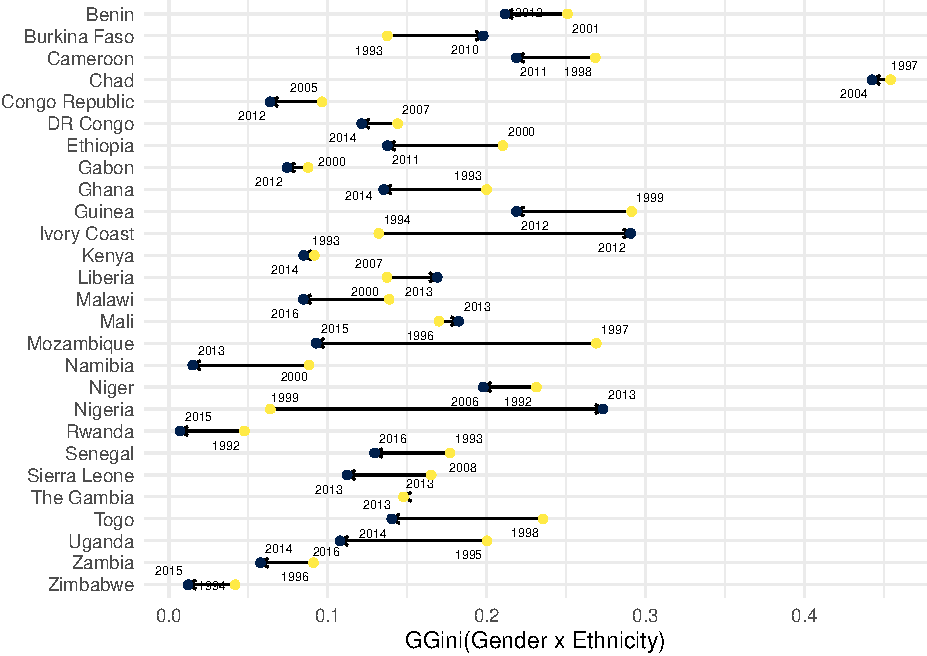
\includegraphics{horizontal_inequality_files/figure-latex/trends-eth-1} \caption[ref:foo]{ref:foo}\label{fig:trends-eth}
\floatfoot{A Figure note.} \end{figure}




\begin{figure}
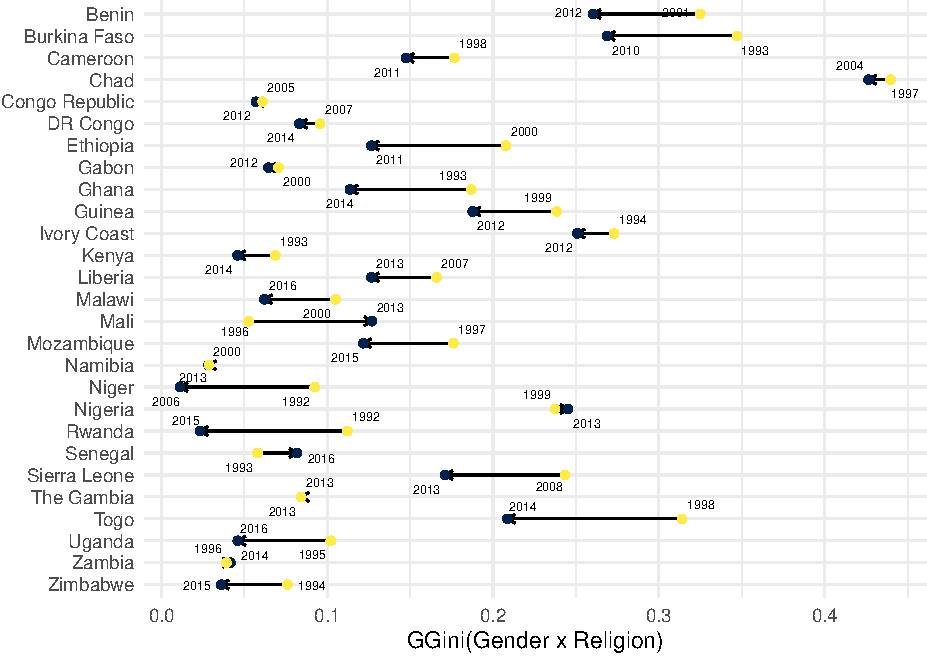
\includegraphics{horizontal_inequality_files/figure-latex/trends-rel-1} \caption[ref:fig-trends-rel]{ref:fig-trends-rel}\label{fig:trends-rel}
\floatfoot{(ref:note-trends-rel)} \end{figure}




\begin{figure}
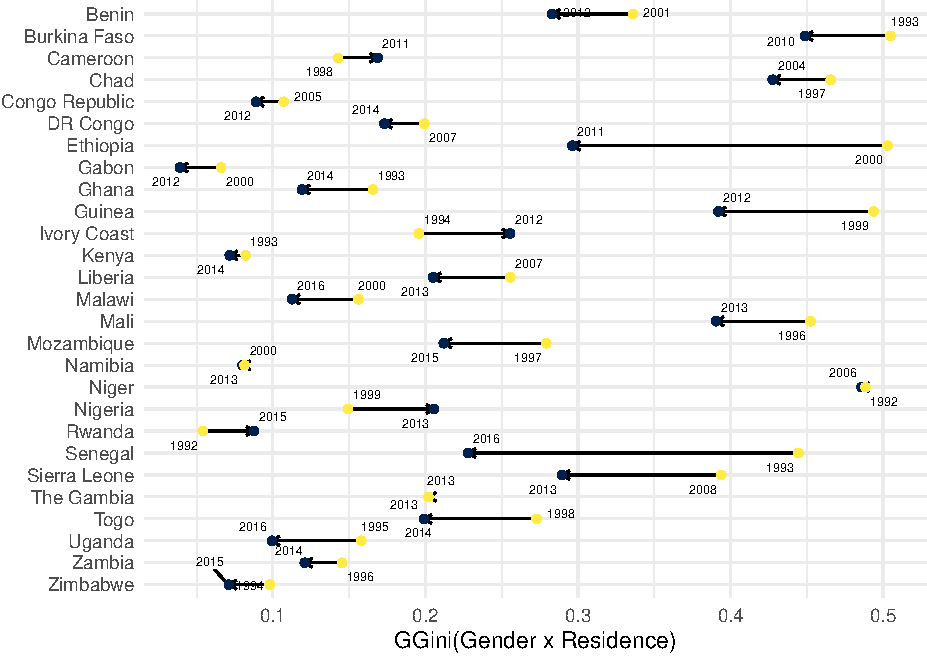
\includegraphics{horizontal_inequality_files/figure-latex/trends-res-1} \caption[ref:fig-trends-res]{ref:fig-trends-res}\label{fig:trends-res}
\floatfoot{(ref:note-trends-res)} \end{figure}

\begin{Shaded}
\begin{Highlighting}[]
\NormalTok{df\_nest }\SpecialCharTok{\%\textgreater{}\%} 
  \FunctionTok{ggplot}\NormalTok{(}\FunctionTok{aes}\NormalTok{(}\AttributeTok{x=}\NormalTok{gg\_gen, }\AttributeTok{y=}\FunctionTok{unlist}\NormalTok{(res\_gen\_ratio))) }\SpecialCharTok{+} 
  \FunctionTok{geom\_point}\NormalTok{() }\SpecialCharTok{+} 
  \FunctionTok{stat\_cor}\NormalTok{(}\AttributeTok{method =} \StringTok{"pearson"}\NormalTok{) }\SpecialCharTok{+}
  \FunctionTok{labs}\NormalTok{(}\AttributeTok{caption =} \StringTok{"Groups: Gender"}\NormalTok{, }\AttributeTok{x=}\StringTok{"GGini"}\NormalTok{, }\AttributeTok{y=}\StringTok{"Ratio lowest/highest"}\NormalTok{)}
\end{Highlighting}
\end{Shaded}

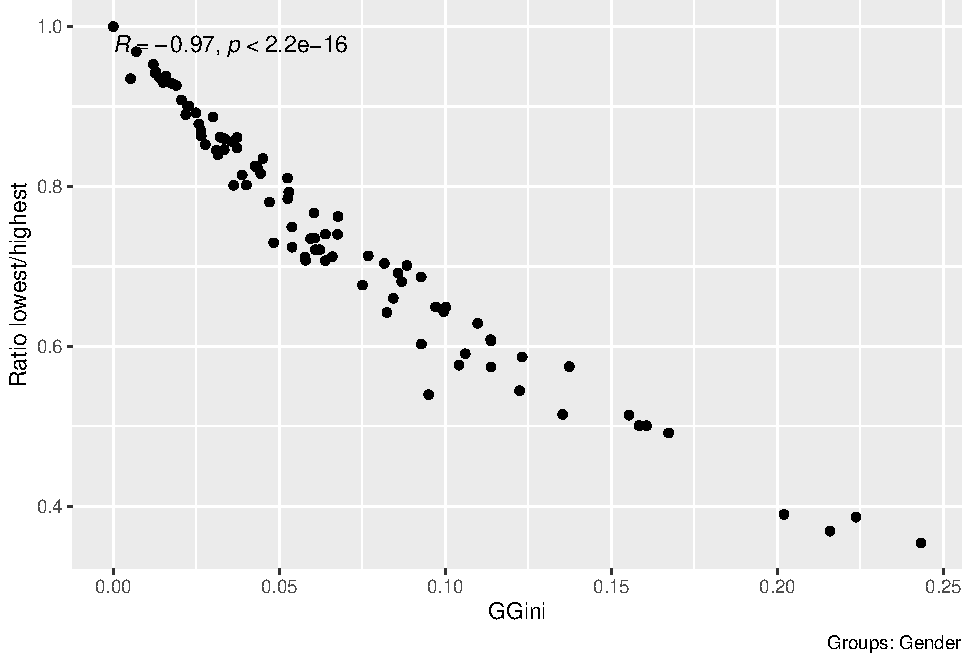
\includegraphics{horizontal_inequality_files/figure-latex/unnamed-chunk-1-1}

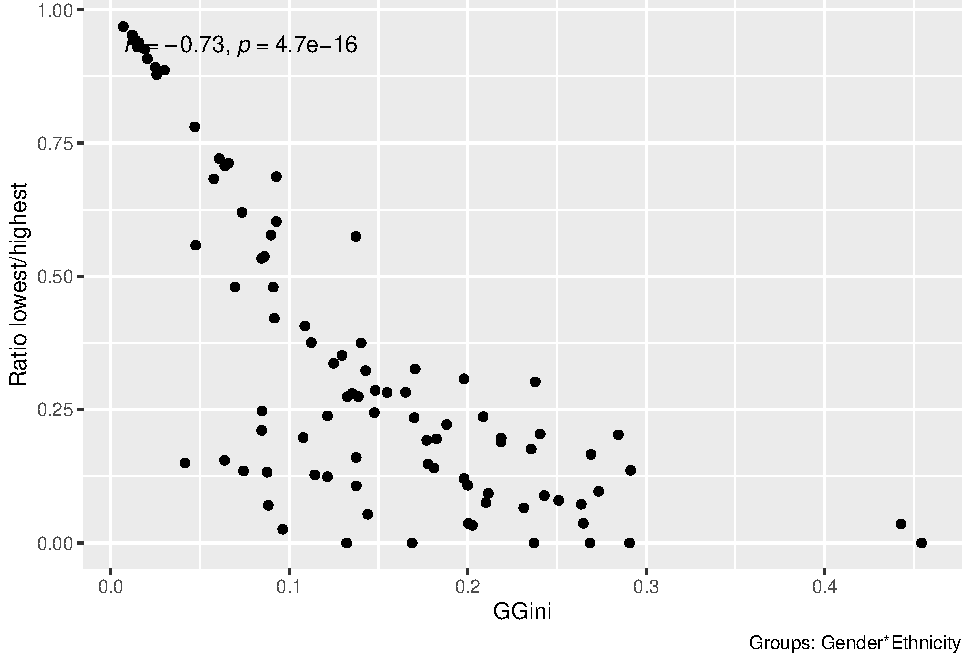
\includegraphics{horizontal_inequality_files/figure-latex/gender-cor-1}

\hypertarget{conclusion}{%
\section{Conclusion}\label{conclusion}}

testing a citation (Fields, 2003)

\clearpage

\hypertarget{references}{%
\section*{References}\label{references}}
\addcontentsline{toc}{section}{References}

\hypertarget{refs}{}
\begin{CSLReferences}{1}{0}
\leavevmode\hypertarget{ref-Fields2003}{}%
Fields, G. S. (2003). \emph{{Accounting for Income Inequality and its Change: A New Method, with Application to the Distribution of Earnings in the United States}} (Vol. 22, pp. 1--38). Emerald Group Publishing Limited. \url{https://doi.org/10.1016/S0147-9121(03)22001-X}

\end{CSLReferences}

\appendix
\clearpage

\hypertarget{group-gini-results}{%
\section{Group Gini Results}\label{group-gini-results}}

\begin{longtable}[t]{rrrrrrrr}
\caption{\label{tab:overview}Intersectional Group Gini Indices by Year and Country}\\
\toprule
year & gender & religion & ethnicity & residence & gen*rel & gen*eth & gen*res\\
\midrule
\endfirsthead
\caption[]{\label{tab:overview}Intersectional Group Gini Indices by Year and Country \textit{(continued)}}\\
\toprule
year & gender & religion & ethnicity & residence & gen*rel & gen*eth & gen*res\\
\midrule
\endhead

\endfoot
\bottomrule
\endlastfoot
\addlinespace[0.3em]
\multicolumn{8}{l}{\textbf{Benin}}\\
\hspace{1em}2001 & 0.16 & 0.27 & 0.15 & 0.16 & 0.33 & 0.25 & 0.34\\
\hspace{1em}2012 & 0.11 & 0.21 & 0.14 & 0.11 & 0.26 & 0.21 & 0.28\\
\addlinespace[0.3em]
\multicolumn{8}{l}{\textbf{Burkina Faso}}\\
\hspace{1em}1993 & 0.06 & 0.32 & 0.10 & 0.06 & 0.35 & 0.14 & 0.50\\
\hspace{1em}1999 & 0.16 & 0.30 & 0.16 & 0.16 & 0.36 & 0.26 & 0.59\\
\hspace{1em}2003 & 0.12 & 0.26 & 0.16 & 0.12 & 0.32 & 0.24 & 0.54\\
\hspace{1em}2010 & 0.10 & 0.22 & 0.14 & 0.10 & 0.27 & 0.20 & 0.45\\
\addlinespace[0.3em]
\multicolumn{8}{l}{\textbf{Cameroon}}\\
\hspace{1em}1998 & 0.04 & 0.16 & 0.26 & 0.04 & 0.18 & 0.27 & 0.14\\
\hspace{1em}2004 & 0.05 & 0.14 & 0.22 & 0.05 & 0.16 & 0.24 & 0.16\\
\hspace{1em}2011 & 0.04 & 0.13 & 0.21 & 0.04 & 0.15 & 0.22 & 0.17\\
\addlinespace[0.3em]
\multicolumn{8}{l}{\textbf{Chad}}\\
\hspace{1em}1997 & 0.24 & 0.33 & 0.33 & 0.24 & 0.44 & 0.45 & 0.47\\
\hspace{1em}2004 & 0.22 & 0.33 & 0.35 & 0.22 & 0.43 & 0.44 & 0.43\\
\addlinespace[0.3em]
\multicolumn{8}{l}{\textbf{Congo Republic}}\\
\hspace{1em}2005 & 0.04 & 0.03 & 0.07 & 0.04 & 0.06 & 0.10 & 0.11\\
\hspace{1em}2012 & 0.04 & 0.03 & 0.04 & 0.04 & 0.06 & 0.06 & 0.09\\
\addlinespace[0.3em]
\multicolumn{8}{l}{\textbf{Democratic Republic of the Congo}}\\
\hspace{1em}2007 & 0.09 & 0.01 & 0.09 & 0.09 & 0.10 & 0.14 & 0.20\\
\hspace{1em}2014 & 0.08 & 0.01 & 0.07 & 0.08 & 0.08 & 0.12 & 0.17\\
\addlinespace[0.3em]
\multicolumn{8}{l}{\textbf{Ethiopia}}\\
\hspace{1em}2000 & 0.09 & 0.15 & 0.13 & 0.09 & 0.21 & 0.21 & 0.50\\
\hspace{1em}2005 & 0.12 & 0.12 & 0.11 & 0.12 & 0.20 & 0.20 & 0.43\\
\hspace{1em}2011 & 0.09 & 0.07 & 0.07 & 0.09 & 0.13 & 0.14 & 0.30\\
\addlinespace[0.3em]
\multicolumn{8}{l}{\textbf{Gabon}}\\
\hspace{1em}2000 & 0.03 & 0.05 & 0.08 & 0.03 & 0.07 & 0.09 & 0.07\\
\hspace{1em}2012 & 0.02 & 0.05 & 0.07 & 0.02 & 0.06 & 0.07 & 0.04\\
\addlinespace[0.3em]
\multicolumn{8}{l}{\textbf{Ghana}}\\
\hspace{1em}1993 & 0.05 & 0.13 & 0.17 & 0.05 & 0.19 & 0.20 & 0.17\\
\hspace{1em}1998 & 0.06 & 0.13 & 0.14 & 0.06 & 0.17 & 0.18 & 0.14\\
\hspace{1em}2003 & 0.07 & 0.12 & 0.14 & 0.07 & 0.17 & 0.18 & 0.15\\
\hspace{1em}2008 & 0.05 & 0.10 & 0.12 & 0.05 & 0.13 & 0.15 & 0.13\\
\hspace{1em}2014 & 0.04 & 0.08 & 0.12 & 0.04 & 0.11 & 0.14 & 0.12\\
\addlinespace[0.3em]
\multicolumn{8}{l}{\textbf{Guinea}}\\
\hspace{1em}1999 & 0.20 & 0.07 & 0.14 & 0.20 & 0.24 & 0.29 & 0.49\\
\hspace{1em}2005 & 0.22 & 0.08 & 0.10 & 0.22 & 0.26 & 0.28 & 0.47\\
\hspace{1em}2012 & 0.16 & 0.06 & 0.11 & 0.16 & 0.19 & 0.22 & 0.39\\
\addlinespace[0.3em]
\multicolumn{8}{l}{\textbf{Ivory Coast}}\\
\hspace{1em}1994 & 0.00 & 0.27 & 0.13 & 0.00 & 0.27 & 0.13 & 0.20\\
\hspace{1em}1999 & 0.11 & 0.25 & 0.24 & 0.11 & 0.30 & 0.24 & 0.26\\
\hspace{1em}2012 & 0.11 & 0.20 & 0.25 & 0.11 & 0.25 & 0.29 & 0.26\\
\addlinespace[0.3em]
\multicolumn{8}{l}{\textbf{Kenya}}\\
\hspace{1em}1993 & 0.04 & 0.04 & 0.07 & 0.04 & 0.07 & 0.09 & 0.08\\
\hspace{1em}1998 & 0.03 & 0.02 & 0.05 & 0.03 & 0.05 & 0.07 & 0.08\\
\hspace{1em}2003 & 0.02 & 0.06 & 0.11 & 0.02 & 0.07 & 0.11 & 0.08\\
\hspace{1em}2009 & 0.02 & 0.05 & 0.08 & 0.02 & 0.06 & 0.08 & 0.08\\
\hspace{1em}2014 & 0.01 & 0.04 & 0.08 & 0.01 & 0.05 & 0.08 & 0.07\\
\addlinespace[0.3em]
\multicolumn{8}{l}{\textbf{Liberia}}\\
\hspace{1em}2007 & 0.14 & 0.05 & 0.00 & 0.14 & 0.17 & 0.14 & 0.26\\
\hspace{1em}2013 & 0.10 & 0.04 & 0.11 & 0.10 & 0.13 & 0.17 & 0.20\\
\addlinespace[0.3em]
\multicolumn{8}{l}{\textbf{Malawi}}\\
\hspace{1em}2000 & 0.06 & 0.06 & 0.11 & 0.06 & 0.11 & 0.14 & 0.16\\
\hspace{1em}2004 & 0.03 & 0.05 & 0.10 & 0.03 & 0.07 & 0.11 & 0.12\\
\hspace{1em}2010 & 0.02 & 0.05 & 0.08 & 0.02 & 0.06 & 0.09 & 0.09\\
\hspace{1em}2016 & 0.03 & 0.04 & 0.07 & 0.03 & 0.06 & 0.08 & 0.11\\
\addlinespace[0.3em]
\multicolumn{8}{l}{\textbf{Mali}}\\
\hspace{1em}1996 & 0.00 & 0.05 & 0.17 & 0.00 & 0.05 & 0.17 & 0.45\\
\hspace{1em}2001 & 0.00 & 0.06 & 0.13 & 0.00 & 0.06 & 0.13 & 0.42\\
\hspace{1em}2006 & 0.14 & 0.05 & 0.09 & 0.14 & 0.17 & 0.19 & 0.42\\
\hspace{1em}2013 & 0.11 & 0.02 & 0.11 & 0.11 & 0.13 & 0.18 & 0.39\\
\addlinespace[0.3em]
\multicolumn{8}{l}{\textbf{Mozambique}}\\
\hspace{1em}1997 & 0.10 & 0.11 & 0.20 & 0.10 & 0.18 & 0.27 & 0.28\\
\hspace{1em}2003 & 0.09 & 0.08 & 0.00 & 0.09 & 0.16 & 0.09 & 0.29\\
\hspace{1em}2011 & 0.06 & 0.08 & 0.21 & 0.06 & 0.11 & 0.24 & 0.23\\
\hspace{1em}2015 & 0.09 & 0.04 & 0.00 & 0.09 & 0.12 & 0.09 & 0.21\\
\addlinespace[0.3em]
\multicolumn{8}{l}{\textbf{Namibia}}\\
\hspace{1em}2000 & 0.01 & 0.02 & 0.07 & 0.01 & 0.03 & 0.09 & 0.08\\
\hspace{1em}2007 & 0.03 & 0.02 & 0.00 & 0.03 & 0.04 & 0.03 & 0.09\\
\hspace{1em}2013 & 0.02 & 0.02 & 0.00 & 0.02 & 0.03 & 0.02 & 0.08\\
\addlinespace[0.3em]
\multicolumn{8}{l}{\textbf{Niger}}\\
\hspace{1em}1992 & 0.05 & 0.04 & 0.21 & 0.05 & 0.09 & 0.23 & 0.49\\
\hspace{1em}1998 & 0.03 & 0.02 & 0.18 & 0.03 & 0.05 & 0.21 & 0.46\\
\hspace{1em}2006 & 0.00 & 0.01 & 0.20 & 0.00 & 0.01 & 0.20 & 0.49\\
\addlinespace[0.3em]
\multicolumn{8}{l}{\textbf{Nigeria}}\\
\hspace{1em}1999 & 0.06 & 0.21 & 0.00 & 0.06 & 0.24 & 0.06 & 0.15\\
\hspace{1em}2003 & 0.07 & 0.23 & 0.00 & 0.07 & 0.26 & 0.07 & 0.17\\
\hspace{1em}2008 & 0.06 & 0.20 & 0.25 & 0.06 & 0.23 & 0.26 & 0.17\\
\hspace{1em}2013 & 0.07 & 0.21 & 0.25 & 0.07 & 0.25 & 0.27 & 0.21\\
\addlinespace[0.3em]
\multicolumn{8}{l}{\textbf{Rwanda}}\\
\hspace{1em}1992 & 0.01 & 0.11 & 0.04 & 0.01 & 0.11 & 0.05 & 0.05\\
\hspace{1em}2005 & 0.02 & 0.04 & 0.00 & 0.02 & 0.05 & 0.02 & 0.09\\
\hspace{1em}2008 & 0.03 & 0.04 & 0.00 & 0.03 & 0.05 & 0.03 & 0.09\\
\hspace{1em}2010 & 0.01 & 0.02 & 0.00 & 0.01 & 0.03 & 0.01 & 0.08\\
\hspace{1em}2015 & 0.01 & 0.02 & 0.00 & 0.01 & 0.02 & 0.01 & 0.09\\
\addlinespace[0.3em]
\multicolumn{8}{l}{\textbf{Senegal}}\\
\hspace{1em}1993 & 0.06 & 0.00 & 0.15 & 0.06 & 0.06 & 0.18 & 0.44\\
\hspace{1em}1997 & 0.08 & 0.00 & 0.10 & 0.08 & 0.08 & 0.14 & 0.40\\
\hspace{1em}2005 & 0.08 & 0.05 & 0.11 & 0.08 & 0.12 & 0.15 & 0.34\\
\hspace{1em}2011 & 0.08 & 0.04 & 0.13 & 0.08 & 0.12 & 0.17 & 0.30\\
\hspace{1em}2014 & 0.05 & 0.04 & 0.10 & 0.05 & 0.08 & 0.12 & 0.23\\
\hspace{1em}2016 & 0.05 & 0.03 & 0.11 & 0.05 & 0.08 & 0.13 & 0.23\\
\addlinespace[0.3em]
\multicolumn{8}{l}{\textbf{Sierra Leone}}\\
\hspace{1em}2008 & 0.11 & 0.17 & 0.07 & 0.11 & 0.24 & 0.17 & 0.39\\
\hspace{1em}2013 & 0.09 & 0.11 & 0.04 & 0.09 & 0.17 & 0.11 & 0.29\\
\addlinespace[0.3em]
\multicolumn{8}{l}{\textbf{The Gambia}}\\
\hspace{1em}2013 & 0.06 & 0.03 & 0.12 & 0.06 & 0.08 & 0.15 & 0.20\\
\addlinespace[0.3em]
\multicolumn{8}{l}{\textbf{Togo}}\\
\hspace{1em}1998 & 0.17 & 0.24 & 0.13 & 0.17 & 0.31 & 0.24 & 0.27\\
\hspace{1em}2014 & 0.10 & 0.16 & 0.07 & 0.10 & 0.21 & 0.14 & 0.20\\
\addlinespace[0.3em]
\multicolumn{8}{l}{\textbf{Uganda}}\\
\hspace{1em}1995 & 0.08 & 0.04 & 0.16 & 0.08 & 0.10 & 0.20 & 0.16\\
\hspace{1em}2001 & 0.06 & 0.03 & 0.00 & 0.06 & 0.08 & 0.06 & 0.14\\
\hspace{1em}2006 & 0.05 & 0.04 & 0.00 & 0.05 & 0.08 & 0.05 & 0.12\\
\hspace{1em}2011 & 0.03 & 0.03 & 0.11 & 0.03 & 0.05 & 0.12 & 0.12\\
\hspace{1em}2016 & 0.03 & 0.03 & 0.09 & 0.03 & 0.05 & 0.11 & 0.10\\
\addlinespace[0.3em]
\multicolumn{8}{l}{\textbf{Zambia}}\\
\hspace{1em}1996 & 0.04 & 0.00 & 0.07 & 0.04 & 0.04 & 0.09 & 0.15\\
\hspace{1em}2002 & 0.04 & 0.01 & 0.06 & 0.04 & 0.05 & 0.09 & 0.14\\
\hspace{1em}2007 & 0.05 & 0.01 & 0.05 & 0.05 & 0.05 & 0.07 & 0.14\\
\hspace{1em}2014 & 0.04 & 0.01 & 0.04 & 0.04 & 0.04 & 0.06 & 0.12\\
\addlinespace[0.3em]
\multicolumn{8}{l}{\textbf{Zimbabwe}}\\
\hspace{1em}1994 & 0.03 & 0.06 & 0.01 & 0.03 & 0.08 & 0.04 & 0.10\\
\hspace{1em}1999 & 0.02 & 0.04 & 0.00 & 0.02 & 0.05 & 0.02 & 0.09\\
\hspace{1em}2006 & 0.02 & 0.03 & 0.00 & 0.02 & 0.04 & 0.02 & 0.07\\
\hspace{1em}2011 & 0.02 & 0.02 & 0.00 & 0.02 & 0.04 & 0.02 & 0.06\\
\hspace{1em}2015 & 0.01 & 0.02 & 0.00 & 0.01 & 0.04 & 0.01 & 0.07\\*
\end{longtable}

\hypertarget{test-two}{%
\section{Test two}\label{test-two}}

another appendix chapter


\end{document}
